\subsection{Syllable resource classes and delays}
\label{sec:core-ug-isa-syl-classes}

Some syllables take more than one cycle to complete. In this case, they are
always pipelined; no multi-cycle syllable will stall the rest of the bundle.
While this is good for performance, it does require the attention of the
programmer in order to write properly functioning code.

In addition, not all pipelanes support execution of all syllables, and as such, 
requirements are imposed on the position of certain syllables within a bundle in 
the binary. The assembler will normally ensure that these requirements are met, 
unlike the delay requirements, which it cannot detect. However, it is still 
important for the user to know them in order to be able to write assembly.

It is also important that the assembler is configured in the same way as the
core. If there are discrepancies, the assembler may still output binaries that
the core cannot execute. If this happens, the core will produce an
\trap{INVALID_OP} trap, with the index of the offending pipelane as the trap
argument.

There are five distinguishable classes of syllables. These classes are ALU,
multiply, memory, branch and long immediate.


\subsubsection{ALU class}
\label{sec:core-ug-isa-syl-classes-alu}

ALU syllables are the basic \rvex{} instructions. They can be processed by every
lane. In the default pipeline and forwarding configuration of the \rvex{}, their
results are available after a single cycle. That is, the bundle immediately
following can use their results.


\subsubsection{Multiply class}
\label{sec:core-ug-isa-syl-classes-mul}

Multiply syllables are only allowed in lanes that are configured to have a
multiplier. This configuration is done at design time using generics. In the
default configuration, every lane has a multiplication unit.

In the default pipeline and forwarding configuration of the \rvex{}, multiply 
instructions are two-cycle pipelined. That is, two bundle boundaries are needed 
between the syllable producing the value and a syllable that uses it.


\subsubsection{Memory class}
\label{sec:core-ug-isa-syl-classes-mem}

Memory syllables are only allowed in lanes that are configured to have a memory 
unit. In addition, in most configurations, only one memory unit can be active 
per context at a time, even if multiple are available. This is due to the fact 
the data cache can only perform one operation per cycle per context. In theory, 
it is still permissible in such a system to perform a single memory operation 
and a single control register operation at the same time, but there is currently
no toolchain support for this.

In the default pipeline and forwarding configuration of the \rvex{}, memory load
instructions are two-cycle pipelined. That is, two bundle boundaries are needed 
between a load syllable and the first syllable that uses the value. However,
there is no store to load delay; if a bundle with a load of a certain address
immediately follows a bundle that stores a value at that address, the newly
written value is loaded.


\subsubsection{Branch class}
\label{sec:core-ug-isa-syl-classes-br}

All syllables that affect the program counter are considered branch syllables. 
Only one branch syllable is permitted per cycle, and in almost all design-time 
core configurations, it must be the last syllable in a bundle.

In the previous \rvex{} version, a delay was needed between a syllable producing
a branch register or link register value and branch operations. This is not the
case in the default pipeline and forwarding configuration of this \rvex{}
version, as the ALU and branch operations are initiated in the same pipeline
stage.


\subsubsection{Long immediate class}
\label{sec:core-ug-isa-syl-classes-limm}

Sometimes, one syllable does not contain enough information for one pipelane to 
execute. The only time when this happens in the \rvex{} processor is when an 
immediate outside the range -256..255 is to be specified. For this purpose, 
\insn{LIMMH} syllables exist. These syllables perform no operation in their own 
pipelane, but instead send 23 additional immediate bits to another lane, which 
allows a 32-bit immediate to be used in a single cycle.

Any ALU, multiply or memory syllable that supports an immediate can receive a
long immediate. However, long immediates can \textit{not} be used to extend the
branch offset field.

\insn{LIMMH} syllables are automatically inferred by the assembler. However,
each \insn{LIMMH} syllable inferred means that one less functional syllable can
be scheduled in a single bundle. In addition, a certain pipelane can not `send'
a long immediate to any other pipelane.

The \rvex{} supports two routes for long immediates to take. They are called
`long immediate from neighbor' and `long immediate from previous pair'. One or
both of these methods may be enabled at design time using generics.

\paragraph*{Long immediate from neighbor}

This is the most common route, as it is supported in all \rvex{} configurations. 
This allows all pipelanes to forward a long immediate to their immediate 
neighbor within a pair of pipelanes. This is depicted in 
Figure~\ref{fig:core-ug-isa-syl-classes-limm-previous} for an 8-way \rvex{} 
processor.

\begin{figure}[h!]
  \centering
  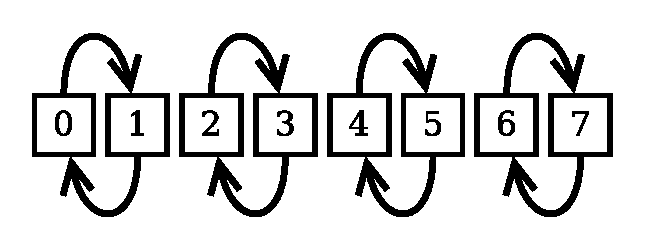
\includegraphics[scale=0.6]{assets/long-immediate-fwding/neighbor}
  \caption{Long immediate from neighbor routing.}
  \label{fig:core-ug-isa-syl-classes-limm-neighbor}
\end{figure}

\paragraph*{Long immediate from previous pair}

This provides an alternative place where a long immediate can be placed for 
lanes 2 and up; when this route is enabled lane $n$ can send a long immediate to 
lane $n+2$. This is depicted in 
Figure~\ref{fig:core-ug-isa-syl-classes-limm-previous} for an 8-way \rvex{} 
processor. However, due to limitations in the instruction fetch unit, this 
system is incompatible with the stop bit system. For these reasons, it can only 
be effectively used in cores with at least four lanes that are not configured 
to support stop bits.

\begin{figure}[h!]
  \centering
  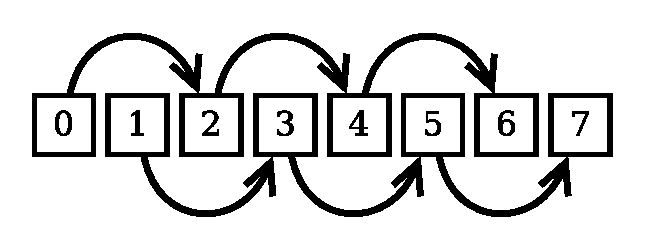
\includegraphics[scale=0.6]{assets/long-immediate-fwding/previous}
  \caption{Long immediate from previous pair routing.}
  \label{fig:core-ug-isa-syl-classes-limm-previous}
\end{figure}

